\documentclass[12pt,titlepage]{article}
\usepackage[margin=1.25in]{geometry}
\usepackage{graphicx,amsmath,minted}

%% Variables definition
\newcommand{\vSubject}{Object Oriented Programming}
\newcommand{\vSubtitle}{Class Relationship}
\newcommand{\vName}{Dicha Zelianivan Arkana}
\newcommand{\vNIM}{2241720002}
\newcommand{\vClass}{2i}
\newcommand{\vDepartment}{Information Technology}
\newcommand{\vStudyProgram}{D4 Informatics Engineering}

%% [START] Tikz related stuff
\usepackage{tikz}
\usetikzlibrary{svg.path,calc,shapes.geometric,shapes.misc}
\tikzstyle{terminator} = [rectangle, draw, text centered, rounded corners = 1em, minimum height=2em]
\tikzstyle{preparation} = [chamfered rectangle, chamfered rectangle sep=0.75em, draw, text centered, minimum height = 2em]
\tikzstyle{process} = [rectangle, draw, text centered, minimum height=2em]
\tikzstyle{decision} = [diamond, aspect=2, draw, text centered, minimum height=2em]
\tikzstyle{data}=[trapezium, draw, text centered, trapezium left angle=60, trapezium right angle=120, minimum height=2em]
\tikzstyle{connector} = [line width=0.25mm,->]
%% [END] Tikz related stuff

%% [START] Fancy header related stuff
\usepackage{fancyhdr}
\pagestyle{fancy}
\setlength{\headheight}{15pt} % compensate fancyhdr style
\fancyhead{}
\fancyfoot{}
\fancyfoot[L]{\thepage}
\fancyfoot[R]{\textit{\vSubject - \vSubtitle}}
\renewcommand{\footrulewidth}{0.4pt}% default is 0pt, overline for footer
%% [END] Fancy header related stuff

%% [START] Custom tabular command related stuff
\usepackage{tabularx}
\newcommand{\details}[2]{
    #1 & #2  \\
}
%% [END] Custom tabular command related stuff

%% [START] Figure related stuff
\newcommand{\image}[3][1]{
    \begin{figure}[h]
        \centering
        \includegraphics[#1]{#2}
        \caption{#3}
        \label{#3}
    \end{figure}
}
%% [END] Figure related stuff

\begin{document}
\begin{titlepage}
    \centering
    \vfill
    {\bfseries\LARGE
        \vSubject\\
        \vskip0.25cm
        \vSubtitle
    }
    \vfill
    
\includegraphics[width=6cm]{images/polinema-logo.png}
    \vfill
    {
        \textbf{Name}\\
        \vName\\
        \vskip0.5cm
        \textbf{NIM}\\
        \vNIM\\
        \vskip0.5cm
        \textbf{Class}\\
        \vClass\\
        \vskip0.5cm
        \textbf{Department}\\
        \vDepartment\\
        \vskip0.5cm
        \textbf{Study Program}\\
        \vStudyProgram
    }
\end{titlepage}

\section{Practicum}
\subsection{Questions}
Based on the first practicum, answer these questions:
\begin{enumerate}
    \item {
        On the class \texttt{Processor} and \texttt{Laptop}, there are setter and getter methods.
        What are those used for?

        Those methods are used to get and set the values of the private properties / attributes.
    }
    \item {
        On the class \texttt{Processor} and \texttt{Laptop}, there is a constructor without parameter
        and another one with parameter. What are the differences?

        The first constructor doesn't have any parameter meaning that we don't need to pass anything to the constructor.
        The second constructor requires some arguments to be passed when instantiating.
    }
    \item {
        The class \texttt{Laptop} has two attributes, namely \texttt{brand} and \texttt{proc}. Which of them
        has an object data type?

        The \texttt{proc} has the \texttt{Processor} data type.
    }
    \item {
        Which part of the class \texttt{Laptop} that shows a relation to the class \texttt{Processor}?

        The class \texttt{Laptop} has a relation to the class \texttt{Processor} shown by it having an attribute
        called \texttt{proc} which has the \texttt{Processor} data type.
    }
    \item {
        What is the use of \texttt{proc.info()}?

        It is used to print the information of the processor.
    }
    \item {
        Pay attention to this code:

        \begin{minted}[autogobble,fontsize=\small]{java}
            Laptop l = new Laptop("Thinkpad", p);
        \end{minted}

        What is \texttt{p} in this context?

        \texttt{p} is an object of the \texttt{Processor} class that we've instantiated earlier.

        What happen if that piece of code is modified into

        \begin{minted}[autogobble,fontsize=\small]{java}
            Laptop l = new Laptop("Thinkpad", new Processor("Intel i5", 3));
        \end{minted}

        There will be no difference because we just replaced the instance of the \\
        \texttt{Processor} class with a new instantiation using the same exact arguments.
    }
\end{enumerate}

\pagebreak

\section{Practicum}
\subsection{Questions}
\begin{enumerate}
    \item {
        Which part of the \texttt{Customer} class that shows a relationship between the class \texttt{Car} and \texttt{Driver}?

        The \texttt{Customer} class has a relationship with the \texttt{Car} and \texttt{Driver} class shown by it having
        attributes of the \texttt{Car} and \texttt{Driver} data type.
    }
    \item {
        Why does the method \texttt{calculateDriverFee} and \texttt{calculateCarFee} has a \texttt{days}
        parameter?

        Because we want to calculate the fee based on how many days it being rented. The \texttt{days} parameter
        acts as a parameter.
    }
    \item {
        What is this code used for?

        \begin{minted}[autogobble,fontsize=\small]{java}
            car.calculateCarFee(days);
            driver.calculateDriverFee(days);
        \end{minted}

        Those methods are used to calculate the fee of each car and driver for how many days that has been passed.
    }
    \item {
        What is this code used for?

        \begin{minted}[autogobble,fontsize=\small]{java}
            customer.setCar(car);
            customer.setDriver(driver);
        \end{minted}

        It is used to set both the car and the driver attribute of a customer object.
    }
    \item {
        What is \texttt{customer.calculateTotalFee()} used for?

        It is used to calculate the total fee of a customer.
    }
    \item {
        What is \texttt{customer.getCar().getBrand()} used for?

        It is used to get the brand of the car that a customer has.
    }
\end{enumerate}

\pagebreak

\section{Practicum}
\subsection{Questions}
\begin{enumerate}
    \item {
        What is \texttt{this.trainDriver.info()} and \texttt{this.assistant.info()} used for?

        They're used to get the information of the \texttt{trainDriver} and \texttt{assistant}.
    }
    \item {
        Add these code to the \texttt{main()} method!

        \begin{minted}[autogobble,fontsize=\small]{java}
            Employee trainDriver = new Employee("1234", "Spongebob Squarepants");
            Train train = new Train("New Style", "Business", trainDiver);
            System.out.println(train.info());
        \end{minted}
    }
    \item {
        What is the output of the above code?
    }
    \item {
        Fix the \texttt{Train} so that the program can be run!
    }
\end{enumerate}

\section{Practicum}
\subsection{Questions}
\begin{enumerate}
    \item {
        How many seats are in the Train A?

        There are 10 seats.
    }
    \item {
        What does this code mean?

        \begin{minted}[autogobble,fontsize=\small]{java}
            // ...
            if (this.passenger != null) {
                info += "Passenger: " + passenger.info() + "\n";
            }
            // ...
        \end{minted}

        If the passenger is not null, we add the passenger information to the attribute \texttt{info}.
    }
    \item {
        Why in the method \texttt{setPassenger()} on the class \texttt{Carriage}, the number value is subtracted by 1?

        Because the array index starts from 0 and we want the number value to start from 1.
    }
    \item {
        Instantiate a new object \texttt{budi} with the type \texttt{Passenger}, and then insert that to the
        carriage using \texttt{carriage.setPassenger(budi, 1)}. What happens?

        It adds the new passenger \texttt{budi} to the carriage using the method \texttt{setPassenger}
    }
    \item {
        Modify the program so that new passengers are not allowed to sit on the existing seat!

        \begin{minted}[autogobble,fontsize=\small]{java}
            public void setPassenger(Passenger passenger, int number) {
                Passenger existingPassenger = this.seats[number - 1];
                if (existingPassenger != null) {
                    System.out.println("The seat has been occupied already");
                    return;
                }
                this.seats[number - 1].setPassenger(passenger);
            }
        \end{minted}
    }
\end{enumerate}

\pagebreak

\section{Task}
\begin{itemize}
    \item {
        \large{\textbf{Class Relationship Diagram}}
        \begin{center}
            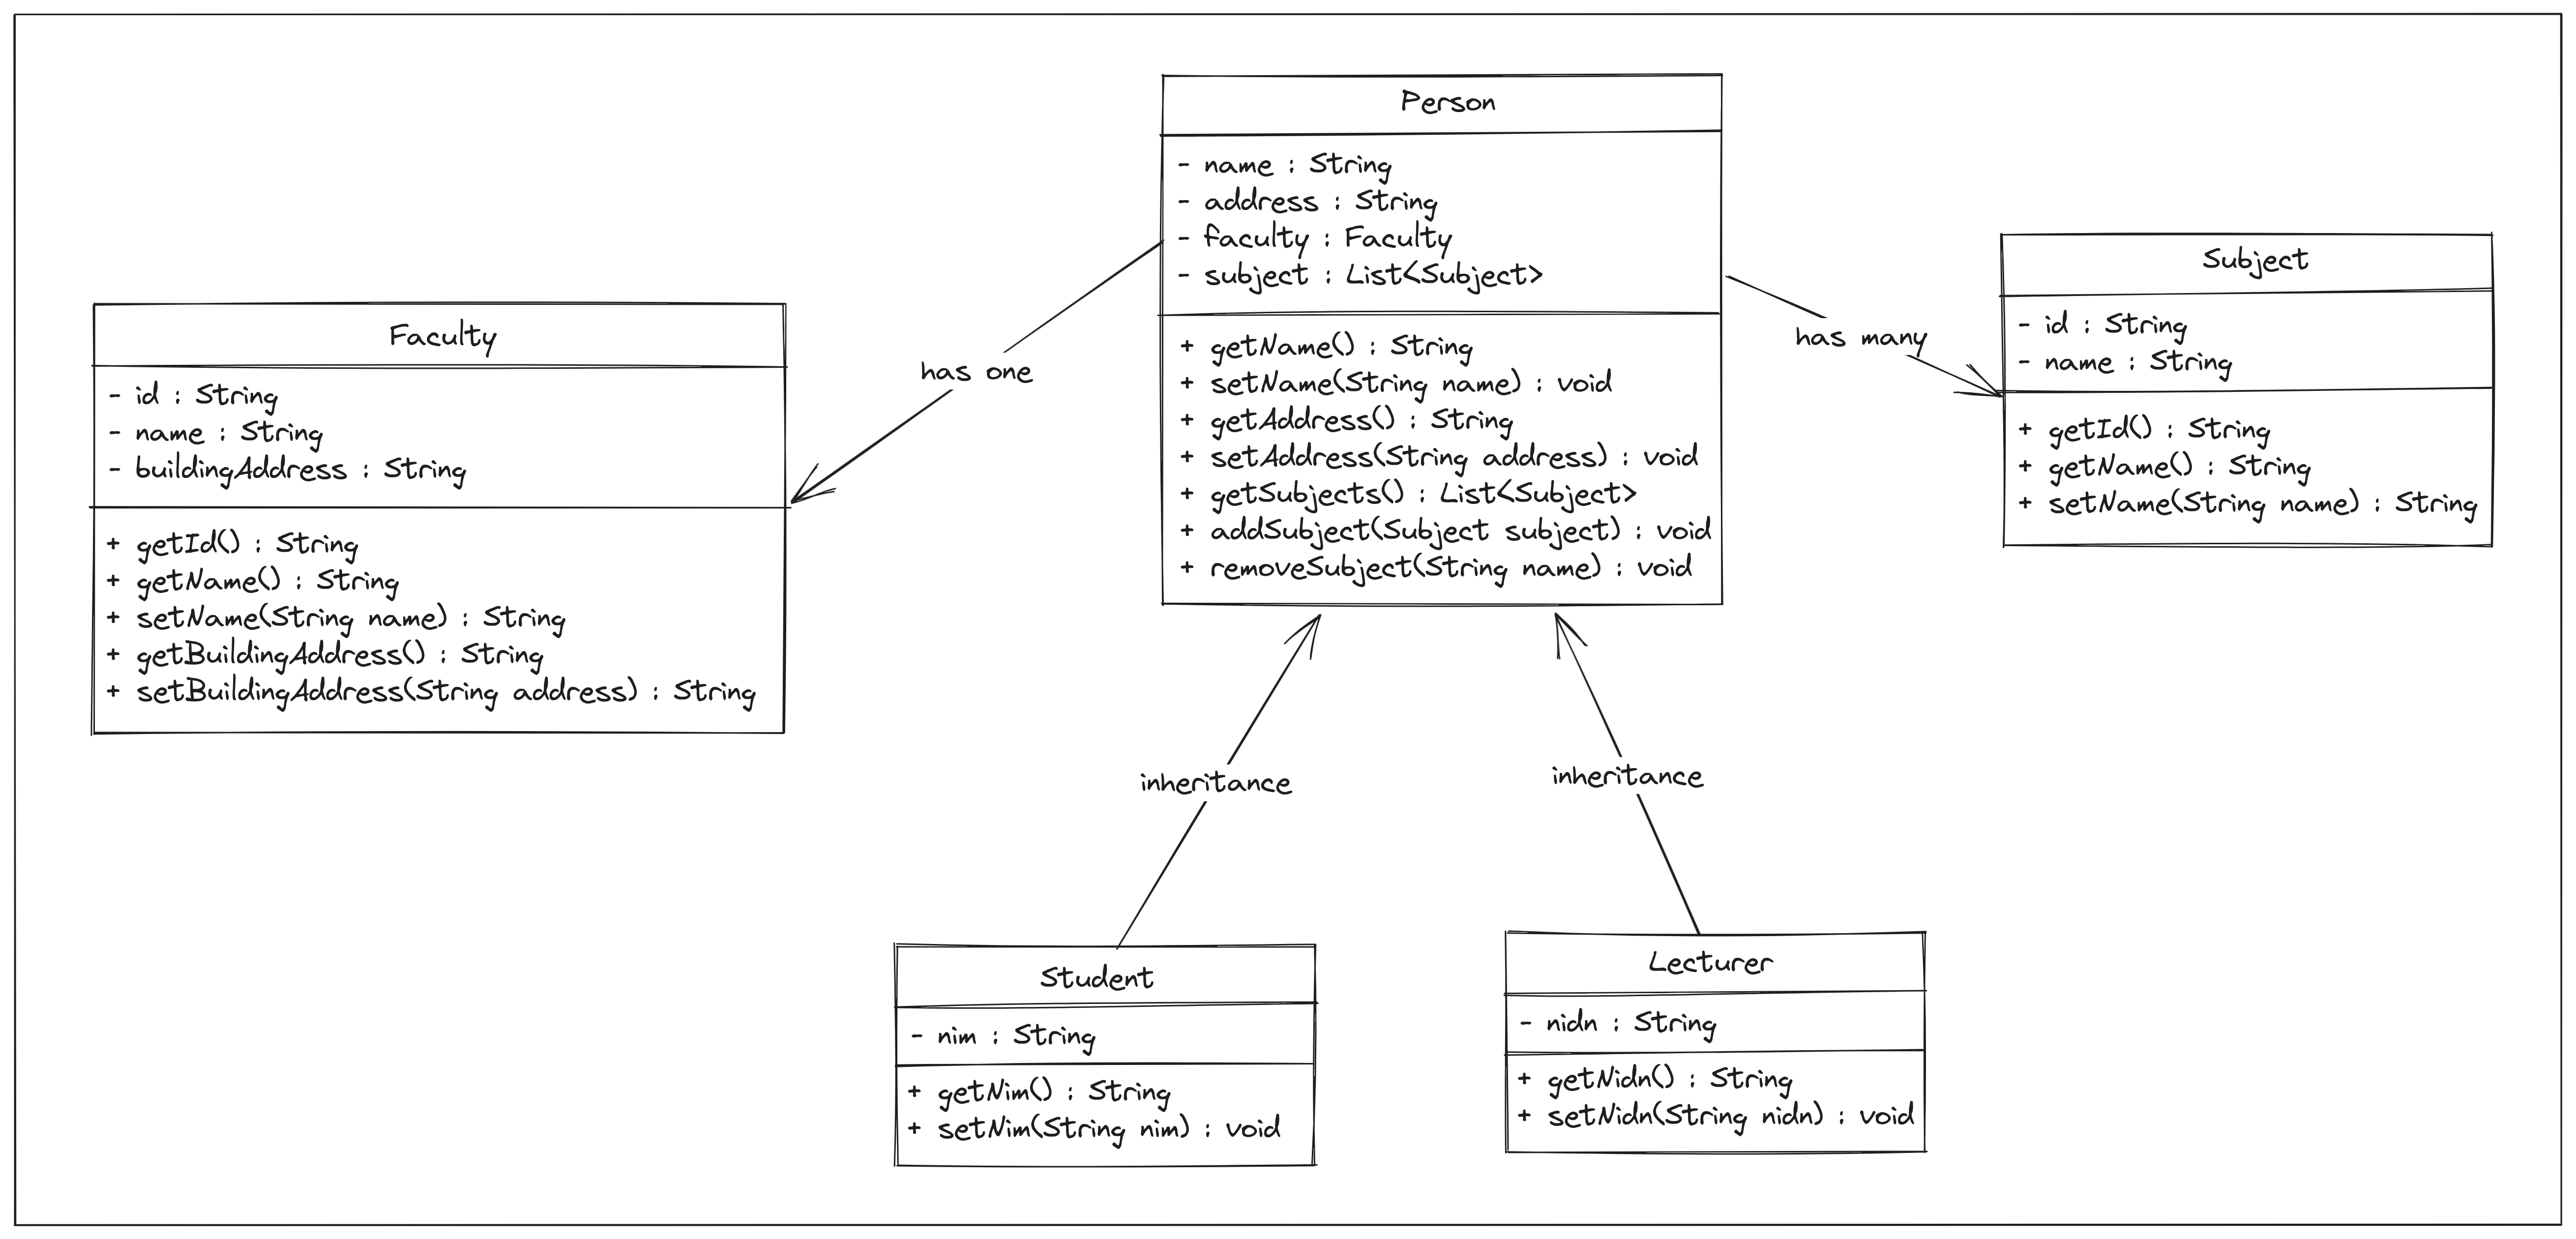
\includegraphics[height=6.8cm]{./images/exodia.png}
        \end{center}
    }
    \item {
        \large{\textbf{Code}}
        \begin{itemize}
            \item {
                \textbf{Main.java}
                \begin{minted}[autogobble,fontsize=\footnotesize]{java}
                    package kuliah;

                    public class Main {
                    public static void main(String[] args) {
                        Subject projectManagement = new Subject("MP", "Project Management");
                        Subject oop = new Subject("OOP", "Object Oriented Programming");

                        Faculty filkom = new Faculty(
                                "FILKOM",
                                "Fakultas Ilmu Komputer",
                                "Building 25"
                        );
                        Faculty fik = new Faculty(
                                "FIK",
                                "Fakultas Industri Kreatif",
                                "Building 26"
                        );
                        Student student = new Student(
                                "2241720002",
                                "Manusia Bernapas",
                                "Bumi Tegal Besar Resident",
                                filkom
                        );
                        student.addSubject(projectManagement);
                        student.addSubject(oop);

                        Lecturer lecturer = new Lecturer(
                                "1234567890",
                                "Dosen",
                                "Something something",
                                fik
                        );
                        lecturer.addSubject(projectManagement);
                        lecturer.addSubject(oop);

                        lecturer.removeSubject("Project Management");

                        System.out.println("Subject for student: " + student.getName());
                        for (Subject subject : student.getSubjects()) {
                            System.out.println("Subject: " + subject.getName());
                        }
                        System.out.println("Student faculty: " + student.getFaculty());
                    }
                }
                \end{minted}
            }
            \item {
                \textbf{Faculty.java}
                \begin{minted}[autogobble,fontsize=\footnotesize]{java}
                    package kuliah;

                    public class Faculty {
                        private String id;
                        private String name;
                        private String buildingAddress;

                        public Faculty(String id, String name, String buildingAddress) {
                            this.id = id;
                            this.name = name;
                            this.buildingAddress = buildingAddress;
                        }

                        public String getId() {
                            return this.id;
                        }

                        public String getName() {
                            return this.name;
                        }

                        public String getBuildingAddress() {
                            return buildingAddress;
                        }

                        public void setBuildingAddress(String buildingAddress) {
                            if (buildingAddress.length() < 3) {
                                throw new IllegalArgumentException(
                                    "Building address can't be shorter than 3 characters"
                                );
                            }
                            this.buildingAddress = buildingAddress;
                        }
                    }
                \end{minted}
            }
            \item {
                \textbf{Person.java}
                \begin{minted}[autogobble,fontsize=\footnotesize]{java}
                    package kuliah;

                    import java.util.List;

                    public class Person {
                        private String name;
                        private String address;
                        private Faculty faculty;
                        private List<Subject> subjects;

                        public Person(String name, String address, Faculty faculty) {
                            this.name = name;
                            this.address = address;
                            this.faculty = faculty;
                        }

                        public String getName() {
                            return name;
                        }

                        public void setName(String name) {
                            if (name.isEmpty()) {
                                throw new IllegalArgumentException("Name can't be empty!");
                            }
                            this.name = name;
                        }

                        public String getAddress() {
                            return address;
                        }

                        public void setAddress(String address) {
                            if (address.length() < 3) {
                                throw new IllegalArgumentException(
                                    "Address can't be shorter than 3 characters"
                                );
                            }
                            this.address = address;
                        }

                        public List<Subject> getSubjects() {
                            return subjects;
                        }

                        public void addSubject(Subject subject) {
                            boolean subjectAlreadyExists = subjects.contains(subject);
                            if (subjectAlreadyExists) {
                                throw new IllegalArgumentException("Subject already exists");
                            }
                            subjects.addLast(subject);
                        }

                        public void removeSubject(String name) {
                            subjects.removeIf(subject -> subject.getName().equals(name));
                        }

                        public Faculty getFaculty() {
                            return faculty;
                        }

                        public void setFaculty(Faculty faculty) {
                            this.faculty = faculty;
                        }
                    }
                \end{minted}
            }
            \item {
                \textbf{Lecturer.java}
                \begin{minted}[autogobble,fontsize=\footnotesize]{java}
                    package kuliah;

                    public class Lecturer extends Person {
                        private String nidn;

                        public Lecturer(String nidn, String name, String address, Faculty faculty) {
                            super(name, address, faculty);
                            this.nidn = nidn;
                        }

                        public String getNidn() {
                            return nidn;
                        }

                        public void setNidn(String nidn) {
                            if (nidn.length() != 10) {
                                throw new IllegalArgumentException("NIDN must be 10 characters long");
                            }
                            this.nidn = nidn;
                        }
                    }
                \end{minted}
            }
            \item {
                \textbf{Student.java}
                \begin{minted}[autogobble,fontsize=\small]{java}
                    package kuliah;

                    public class Student extends Person {
                        private String nim;

                        public Student(String nim, String name, String address, Faculty faculty) {
                            super(name, address, faculty);
                            this.nim = nim;
                        }

                        public String getNim() {
                            return nim;
                        }

                        public void setNim(String nim) {
                            if (nim.length() != 10) {
                                throw new IllegalArgumentException("NIM must be 10 characters long");
                            }
                            this.nim = nim;
                        }
                    }
                \end{minted}
            }
        \end{itemize}
    }
\end{itemize}

\end{document}

